\documentclass[12pt,a4paper]{article}
% !TEX program = xelatex
\usepackage[utf8]{inputenc}
\usepackage[T1]{fontenc}
\usepackage[finnish]{babel}
\usepackage[utf8]{inputenc}
\usepackage{graphicx}
\usepackage{titling}
\usepackage{titlesec}
\usepackage{booktabs}
\usepackage{fancyhdr}
\usepackage{lipsum}
\usepackage{comment}
\usepackage{enumitem}
\usepackage{xcolor}
\usepackage{longtable}
%\usepackage{cite}
\usepackage{pgfgantt}
\usepackage{amsmath, amssymb}
\usepackage{tikz}
\usepackage[margin=1in]{geometry}
\usepackage[backend=biber, style=numeric]{biblatex}
%\usepackage{hyperref}
\usepackage{bookmark}
\usepackage{enumitem}
\usepackage{amsmath}
\usepackage{listings}
\lstset{language=Python, basicstyle=\ttfamily\small, breaklines=true,columns=fullflexible}
\lstset{escapeinside={(*@}{@*)}}
\usepackage{fontspec}
\setmainfont{Arial}
\newfontfamily\stylishfont{Noteworthy}
%\newfontfamily\stylishfont{Zapfino}
%\addbibresource{references.bib}
\usetikzlibrary{calc}
\usepackage{xcolor}

\lstdefinestyle{pidstyle}{
    basicstyle=\ttfamily\footnotesize,
    breaklines=true,
    escapechar=\#, % Define escape character for inline LaTeX commands
    linewidth=\textwidth,
    basicstyle=\ttfamily\scriptsize
}

\renewcommand{\maketitle}{%
  \begin{leftmark}
    \vspace*{\baselineskip} % Add a bit of vertical space

%    \includegraphics[width=4cm]{example-image-a} % Add an image before the title. you will need to replace the image path with your own

%    \vspace{0.5cm} % Add vertical space before title

    \textbf{\fontsize{18}{36}\selectfont \thetitle} % Font Size and Bold Title

     \vspace{0.05cm} % Add vertical space before subtitle
%    \textit{\Large \theauthor}  % Subtitle / Author
    \vspace{\baselineskip} % Add vertical space after subtitle
     \rule{\textwidth}{0.4pt} % Add a horizontal line

   \end{leftmark}
%    \thispagestyle{empty} % Prevent header/footer on the title page
}


% Section Formatting
\titleformat{\section}
  {\normalfont\fontsize{18}{22}\bfseries} % Font and style
  {\thesection}         % Section number
  {1em}                   % Horizontal space after section number
  {}                     % Code before the section name
  []                     % Code after the section name

\titleformat{\subsection}
  {\normalfont\fontsize{14}{18}\bfseries} % Font and style
  {\thesubsection}         % Subsection number
  {1em}                   % Horizontal space after subsection number
  {}                     % Code before the subsection name
  []                     % Code after the subsection name

\setlength{\parindent}{0pt}

\title{Computing platforms (Spring 2025)\newline
week 6}
\author{Juha-Pekka Heikkilä}



\pagestyle{fancy}
\fancyhf{}

\renewcommand{\headrulewidth}{0pt}

\newcommand{\footerline}{\makebox[\textwidth]{\hrulefill}}

\newcommand{\footercontent}{%
    \begin{tabular}{@{}l@{}}
        \footerline \\
        \leftmark \hfill \rlap{\thepage}
    \end{tabular}
}

\fancyfoot[C]{\footercontent}


\newcommand{\exercise}[1]{
    \section*{Tehtävä #1}
    \markboth{Tehtävä #1}{}
}

\addtolength{\hoffset}{-1.75cm}
\addtolength{\textwidth}{3.5cm}
%\addtolength{\voffset}{-3cm}
%\addtolength{\textheight}{6cm}
%\setlength{\parindent}{0pt}



% (a), (b), (c)
\newlist{kohta}{enumerate}{1}
\setlist[kohta,1]{
  label=\textbf{\makebox[1cm][l]{\Huge\text{(\stylishfont\alph*)}}},
  leftmargin=!,
  labelindent=0pt
}

% (1), (2), (3)
\newlist{alakohta}{enumerate}{1}
\setlist[alakohta,1]{
  label=\textbf{\makebox[1cm][l]{\Large\text{(\arabic*)}}},
  leftmargin=!,
  labelindent=0pt
}

% termi: selitys
\newlist{kuvaus}{description}{1}
\setlist[kuvaus]{%
  font=\bfseries\stylishfont,
  labelsep=0.5cm,
  leftmargin=2.5cm,
  style=nextline
}

\newcommand{\korostus}[2][yellow]{\colorbox{#1}{\strut #2}}
%\korostus{Yksi kirjoittaja on jo sisällä}
%\korostus[red]{Lukijan täytyy odottaa jos kirjoittajia on paikalla}
%\korostus[orange]{Tämä osa ei ole suoritettavissa}


\newcommand{\evalslantti}[4][-12]{%
%  \left. #2 \,\right|% ei indeksejä tähän
  \mkern-10mu\raisebox{0pt}[0pt][0pt]{\rotatebox{#1}{$\Big|$}}% vinoviiva päälle
  \mkern3mu{}_{\!#3}^{\!#4}% arvot viivan oikealle puolelle
}



\newcommand{\evalraise}{1.2ex}
\newcommand{\evallow}{1.2ex}

% vino eval-viiva, arvot oikealla (oletus: -12)
% \evalslant[asteet]{lauseke}{ala}{yla}
\newcommand{\evalslant}[4][-12]{%
  \left. #2 \,\right.%
  \mkern-10mu\raisebox{0pt}[0pt][0pt]{\rotatebox{#1}{$\Big|$}}%
  \mkern2mu{}^{\raisebox{\evalraise}{$\scriptstyle #4$}}_{\raisebox{-\evallow}{$\scriptstyle #3$}}%
}

\title{MAT12003 Todennäköisyyslaskenta I — Viikko 5}
\date{}

\begin{document}

\maketitle

\exercise{1}
Olkoon $X$ jatkuva satunnaismuuttuja, jonka tiheysfunktio on 
$$f(x)=\begin{cases}
    \frac{3a^3}{x^{4}},\text{ kun }x\ge a,\\
    0 \text{ muulloin,}
\end{cases}$$
missä $a>0$ on reaalinen parametri. Laske Var$(X)$.

\vspace{0.4cm}


Odotusarvot:
\[
E(X)=\int_a^\infty x\,f(x)\,dx
=3a^3\int_a^\infty x^{-3}\,dx
=3a^3\,\evalslantpre{-\frac{1}{2}x^{-2}}{a}{\infty}
=\frac{3}{2}\,a
\]
\[
E(X^2)=\int_a^\infty x^2\,f(x)\,dx
=3a^3\int_a^\infty x^{-2}\,dx
=3a^3\,\evalslantpre{-x^{-1}}{a}{\infty}
=3a^2
\]
\vspace{0.4cm}

Varianssi (sijoitetaan suoraan vaan määritelmään 6.8):
\[
\operatorname{Var}(X)=E(X^2)-\big(E(X)\big)^2
=3a^2-\Big(\tfrac{3}{2}a\Big)^2
=\frac{3}{4}\,a^2
\]






\pagebreak
\exercise{2}
Olkoot $X$, $Y$ ja $Z$
riippumattomia satunnaismuuttujia, joilla kaikilla on sama odotusarvo $\mu$ ja
varianssi $\sigma^2$. Laske odotusarvo ja varianssi
satunnaismuuttujille (a) $X+2Y+3Z$, (b) $X-Y$, (c) $XY$.

\begin{kohta}

\item $X+2Y+3Z$
\[
\begin{aligned}
    E(X+2Y+3Z) &=\mu+2\mu+3\mu=6\mu \\
    \Var(X+2Y+3Z) &=\sigma^2+4\sigma^2+9\sigma^2=14\sigma^2
\end{aligned}
\]

\item $X-Y$
\[
\begin{aligned}    
E(X-Y)&=\mu-\mu=0 \\
\text{käytetään Huomautus 6.22 ja Lause 6.23:}\\
\Var(X-Y)&=\sigma^2+\sigma^2=2\sigma^2
\end{aligned}
\]

\item $XY$ \\
 (Esimerkki 6.25 ii)
\[
E(XY)=E(X)E(Y)=\mu^2
\]
Sitten: \\
$E(X^2)=\Var(X)+[E(X)]^2=\sigma^2+\mu^2$\\
ja: \\
 $E(Y^2)=\sigma^2+\mu^2$\\
joten
\[
\begin{aligned}
\Var(XY)&=E(X^2Y^2)-[E(XY)]^2\\
&=E(X^2)E(Y^2)-\mu^4\\
&=(\sigma^2+\mu^2)^2-\mu^4\\
&=\sigma^4+2\sigma^2\mu^2
\end{aligned}
\]

\end{kohta}





\pagebreak
\exercise{3}
Tasoon piirretään kolmio, jonka kärkinä ovat origo
sekä $x$- ja $y$-akselilta satunnaisesti valitut pisteet $X$ ja $Y$,
jotka ovat riippumattomia ja noudattavat normaalijakaumaa parametrein
$(0, 1)$. Laske kolmion pinta-alan odotusarvo.
\vspace{0.4cm}

eli kolmio millä kärjet (0,0), (X,0) ja (0,Y), missä X\sim N(0,1) ja 
Y\sim N(0,1) riippumattomia ja kolmion pinta-ala on
\[
A=\frac{|X||Y|}{2}
\]
Riippumattomuudesta seuraa E(|X|\,|Y|)=E(|X|)\,E(|Y|) ja koska X ja Y on
samanlaisia merkitään E(|X|)\,=\,E(|Y|) ja 
E(|X|)\,=\,E(|Y|)\,=\,E(|Z|) kun Z\sim N(0,1) jolloin voidaan kirjoittaa


\[
E(A)=\frac{E(|X|)E(|Y|)}2
=\frac{\bigl(E(|Z|)\bigr)^2}2
\]
ja lasketaan \(E(|Z|)\) (Luento09\_handout lause 5 todistusta apuna käyttäen)
\[
\begin{aligned}
E(|Z|)
&= 2\int_{0}^{\infty} x\;\frac{1}{\sqrt{2\pi}}\,e^\frac{-x^{2}}2\,dx
= \frac{2}{\sqrt{2\pi}}\int_{0}^{\infty} x\,e^\frac{-x^{2}}2\,dx\\[4pt]
&= \frac{2}{\sqrt{2\pi}}\;\evalslantpre{-e^\frac{-x^{2}}2}{0}{\infty}
= \frac{2}{\sqrt{2\pi}}\,(0-(-1))
= \sqrt{\frac{2}{\pi}}
\end{aligned}
\]

Siis
\[
E(A)
=\frac{\bigl(E(|Z|)\bigr)^2}2
=\frac{\left(\sqrt{\frac{2}{\pi}}\right)^{2}}2
=\frac{1}{\pi}\approx 0{,}31831
\]






\pagebreak
\exercise{4}
\begin{enumerate}
    \item [(a)] Todista luentomonisteen Lause 6.20: Olkoot $X$ ja $Y$ satunnaismuuttujia, joiden toiset momentit ovat äärellisiä. Tällöin
$\operatorname{Cov}(X,Y)=E(XY)-E(X)E(Y)$.
    \item[(b)] Todista luentomonisteen Lauseen 6.19 kohta (iii): Jos $X$ ja $Y$ ovat 
satunnaismuuttujia, joilla on äärelliset toiset momentit, niin
$\operatorname{Cov}(aX,Y)=a\operatorname{Cov}(X,Y)$, kun $a \in \mathbb{R}$.
\end{enumerate}


\begin{kohta}
  \item Todista luentomonisteen Lause 6.20: Olkoot $X$ ja $Y$ satunnaismuuttujia, joiden toiset momentit ovat äärellisiä. Tällöin
$\operatorname{Cov}(X,Y)=E(XY)-E(X)E(Y)$. (mulla tuo oli \emph{Lause 6.19})
  \[
    \operatorname{Cov}(X,Y)=E(XY)-E(X)\,E(Y)
  \]
  \textit{Todistus.} Määritelmä 6.17 mukaan
  \[
    \operatorname{Cov}(X,Y)=E\big[(X-E(X))(Y-E(Y))\big]
  \]
  Avataan tulo
  \[
  \begin{aligned}
    \operatorname{Cov}(X,Y)
    &= E(XY) - E\!\big(X\,E(Y)\big) - E\!\big(E(X)\,Y\big) + E\!\big(E(X)\,E(Y)\big)\\
    &= E(XY) - E(Y)\,E(X) - E(X)\,E(Y) + E(X)\,E(Y)\\
    &= E(XY) - E(X)\,E(Y)
  \end{aligned}
  \]

  \item Todista luentomonisteen Lauseen 6.19 kohta (iii): Jos $X$ ja $Y$ ovat 
satunnaismuuttujia, joilla on äärelliset toiset momentit, niin
$\operatorname{Cov}(aX,Y)=a\operatorname{Cov}(X,Y)$, kun $a \in \mathbb{R}$.
(mun materiaaleissa tää oli \linebreak\emph{Lause 6.18 kohta iii})
  
  %\textbf{(Lause 6.19 (iii))} Jos $a\in\mathbb{R}$, niin
  \[
    \operatorname{Cov}(aX,Y)=a\,\operatorname{Cov}(X,Y)
  \]
  \textit{Todistus.} Käytetään määritelmää 6.17 ja lausetta 6.1 (ii)
  \[
  \begin{aligned}
    \operatorname{Cov}(aX,Y)
    &= E\big((aX-E(aX))(Y-E(Y))\big)\\
    &= E\big((aX-a\,E(X))(Y-E(Y))\big)\\
    &= a\,E\big((X-E(X))(Y-E(Y))\big)
     = a\,\operatorname{Cov}(X,Y)
  \end{aligned}
  \]
\end{kohta}





\pagebreak

\exercise{5}
Heitetään kahta 4-sivuista noppaa (jossa silmäluvut 1, 2, 3, 4 ovat yhtä todennäköiset).
Olkoon heittojen tulokset $X$ ja $Y$, ja $S=|X-Y|$. Laske Cov$(X,S)$ ja Corr$(X,S)$. Voitko päätellä tuloksista jotain satunnaismuuttujien $X$ ja $S$ riippuvuudesta?

\vspace{0.4cm}


Ensin S:n ptnf, odotusarvo ja toinen momentti:\\
Mahdollisia pareja on 16. \\

Erotuksen itseisarvon lukumäärät:
\[
\#\{(x,y):|x-y|=s\}=
\begin{array}{c|cccc}
s&0&1&2&3\\\hline
\#&4&6&4&2
\end{array}
\quad\Rightarrow\quad
P(S=s)=\frac{\#}{16}
\]
Tästä saadaan
\[
\begin{aligned}
E(S)&=\frac{0\cdot4+1\cdot6+2\cdot4+3\cdot2}{16}=\frac{20}{16}=\frac54\\
E(S^2)&=\frac{0^2\cdot4+1^2\cdot6+2^2\cdot4+3^2\cdot2}{16}=\frac{40}{16}=\frac52\\
\Var(S)&=E(S^2)-E(S)^2=\frac52-\Big(\frac54\Big)^2=\frac{15}{16}
\end{aligned}
\]

\vspace{0.4cm}

Seuraavaksi samat X:lle\\
Koska $X\sim\mathrm{Tas}\{1,2,3,4\}$
\[
\begin{aligned}
E(X)&=\frac{1+2+3+4}{4}=\frac52\\
E(X^2)&=\frac{1^2+2^2+3^2+4^2}{4}=\frac{15}{2}\\
\Var(X)&=E(X^2)-E(X)^2=\frac{5}{4}
\end{aligned}
\]
\vspace{0.4cm}

Sitten lasketaan $E(S\mid X=x)$ (keskiarvo $Y\in\{1,2,3,4\}$):
\[
\begin{aligned}
E(S\mid X=1)&=\frac14\,(|1-1|+|1-2|+|1-3|+|1-4|)=\frac14(0+1+2+3)=\tfrac32\\
E(S\mid X=2)&=\frac14\,(|2-1|+|2-2|+|2-3|+|2-4|)=\frac14(1+0+1+2)=1\\
E(S\mid X=3)&=\frac14\,(|3-1|+|3-2|+|3-3|+|3-4|)=\frac14(2+1+0+1)=1\\
E(S\mid X=4)&=\frac14\,(|4-1|+|4-2|+|4-3|+|4-4|)=\frac14(3+2+1+0)=\tfrac32
\end{aligned}
\]
josta
\[
E(XS)=E\big(X\,E(S\mid X)\big)
=\frac14\!\left(1\cdot\tfrac32+2\cdot 1+3\cdot 1+4\cdot\tfrac32\right)
=\frac{25}{8}
\]




\pagebreak
nyt on kaikki kovarianssia (Määritelmä 6.17) ja sitten korrelaatiota (Määritelmä 6.20) varten:
\[
\Cov(X,S)=E(XS)-E(X)E(S)
=\frac{25}{8}-\frac52\cdot\frac54=0
\]
\[
\Corr(X,S)=\frac{\Cov(X,S)}{\sqrt{\Var(X)\Var(S)}}=0
\]

\vspace{0.8cm}

\textbf{päätelmä tuloksista satunnaismuuttujien X ja S riippuvuudesta}\\

Vaikka $\Corr(X,S)=0$, muuttujat eivät ole riippumattomia (Huomautus 6.22).\\

Esimerkiksi
\[
P(S=3)=\frac{2}{16}=\frac18,\qquad
P(S=3\mid X=1)=P(|1-Y|=3)=P(Y=4)=\frac14\neq \frac18
\]
Eli X ja S ovat korreloimattomia. Mutta X ja S ovat riippuvaisia.


\pagebreak
\exercise{6}
Korttipakasta nostetaan kortti (takaisin panolla) 320 kertaa. Olkoon $X$ nostettujen herttojen lukumäärä. Arvioi todennäköisyyttä $P(X>100)$ Markovin ja T\v seby\v sevin epäyhtälöillä. (Voit halutessasi laskea myös todennäköisyyden tarkan arvon, esimerkiksi ohjelmistolla, ja verrata arvioita siihen.)

\vspace{0.4cm}

Koska nostot tehdään takaisinpanolla ja hertan todennäköisyys on $p=\tfrac{13}{52}=\tfrac14$, saadaaan
\[
X\sim\mathrm{Bin}(n=320,\ p=\tfrac14),\qquad
E(X)=np=80,\quad
\mathrm{Var}(X)=np(1-p)=60
\]

\begin{kohta}
  \item Markovin epäyhtälö (Lause 7.1)\\
  ei-negatiiviselle $X$:lle ja $a>0$ pätee
  \[
  \begin{aligned}
  &P(X\ge a)\le \frac{E(X)}{a}\\
  \Rightarrow \quad &P(X> 100)\le \frac{80}{100}=0{,}80
  \end{aligned}
  \]


\item T\v{s}eby\v{s}evin epäyhtälö (Lause 7.2)\\


\[
\mu=E(X)=np=80,\qquad \sigma^2=\Var(X)=np(1-p)=60,\quad \sigma=\sqrt{60}
\]

Etsitään siis $P(X>100)$ \\
$X>100 \;\Rightarrow\; X-\mu > 100-80 = 20 \;\Rightarrow\; |X-\mu|\ge 20$
\[
P(X>100)\ \le\ P(|X-\mu|\ge 20)
\]
T\v{s}eby\v{s}evin epäyhtälön mukaan kaikilla $k>0$ pätee
\[
P(|X-\mu|\ge k\sigma)\ \le\ \frac{1}{k^2}
\]
Valitaan\\
\[
k=\dfrac{20}{\sigma}=\dfrac{20}{\sqrt{60}}
\]
Tällöin
\[
P(X>100)\ \le\ P(|X-\mu|\ge 20)
\ \le\ \frac{1}{k^2}
\ =\ \frac{\sigma^2}{20^2}
\ =\ \frac{60}{400}
\ =\ \frac{3}{20}
\ =\ 0{,}15
\]

\item Pythonilla todennäköisyyden tarkka arvo
\begin{verbatim}
    >>> import scipy
    >>> print(1 - scipy.stats.binom.cdf(100, 320, 0.25))
    0.0047979316937751815
\end{verbatim}
\end{kohta}





\pagebreak

\exercise{7}
Olkoon ${X_1, X_2,\ldots, X_{100}}$ otos jakaumasta Tas$(-1,1)$ ja $X=\sum_{k=1}^{100} X_k$. Määritä normaaliapproksimaatiolla likiarvo todennäköisyydelle $P(X>5)$.\\

Vastaus: $0{,}193$.
\vspace{0.4cm}

Tasajakaumalle $\mathrm{Tas}(a,b)$ pätee (Esimerkki 5.16, Esimerkki 6.13)
\[
E(X_k)=\frac{a+b}{2}=0,\qquad
\operatorname{Var}(X_k)=\frac{(b-a)^2}{12}=\frac{(2)^2}{12}=\frac{1}{3}
\]
Silloin
\[
E(X)=100\cdot 0=0,\qquad
\operatorname{Var}(X)=100\cdot \frac{1}{3}=\frac{100}{3},\quad
\operatorname{keskihajonta}(X)=\sqrt{\frac{100}{3}}=\frac{10}{\sqrt{3}}
\]

Keskeisen raja-arvolauseen nojalla (esimerkkiä 7.11 soveltaen)
\[
Z=\frac{X-E(X)}{\sqrt{\operatorname{Var}(X)}}=\frac{X}{\frac{10}{\sqrt{3}}}\ \approx\ N(0,1)
\]
Näin saadaan
\[
P(X>5)\ \approx\ P\!\left(
    Z>\frac{5}{\frac{10}{\sqrt{3}}}
    \right)
=1-\Phi\!\left(\tfrac12\sqrt{3}\right)
\approx 1-\Phi(0.8660)
\approx 0.1932
\]

Siis \(P(X>5)\approx 0{,}193\) normaaliapproksimaatiolla





\pagebreak
\exercise{8}
Asiakkaan ostosten summa pyöristetään lähimpään 5 senttiin. Yhden asiakkaan pyöristys-virheestä liikkeenharjoittajalle koituva tappio on satunnaismuuttuja, joka saa arvot $-2$, $-1$, $0$, $1$, $2$ (yksikkönä sentti) kunkin todennäköisyydellä $\frac{1}{5}$. Olkoon $X$ 10 000 asiakkaan aiheuttama kokonaistappio. Laske normaaliapproksimaatiolla (jatkuvuuskorjausta käyttäen) todennäköisyyden $P(X>2\text{ EUR})$ kolmidesimaalinen likiarvo. \\

Vastaus: 0{,}078.\\


\medskip
Merkitään yhden asiakkaan tappiota T:llä.
\[
P(T=t)=\tfrac15,\qquad t\in\{-2,-1,0,1,2\}
\]
Odotusarvo ja varianssi:
\[
E(T)=\tfrac15(-2-1+0+1+2)=0,\qquad
E(T^2)=\tfrac15(4+1+0+1+4)=2\ \Rightarrow\ \Var(T)=2
\]
Olkoot $T_1,...,T_{10000}$ riippumattomia kuten $T$ ja $X=\sum_{i=1}^{10000}T_i$\\
Tällöin
\[
E(X)=10000\cdot 0=0,\qquad
\Var(X)=10000\cdot 2=20000,\qquad
\sigma_X=\sqrt{20000}=100\sqrt2
\]
\vspace{0.4cm}

Halutaan että $P(X>200)$ koska 2 EUR on 200 senttiä.\\
Käytetään normaaliapproksimaatiota
jatkuvuuskorjauksella (5.1.3 Normaalijakauma ja Esimerkki 5.14)
\[
P(X>200)\approx P\bigl(N>201\bigr),\quad N\sim N\!\bigl(0,\,20000\bigr)
\]
Stnadardoiden saadaan
\[
\begin{aligned}
z=\frac{201-0}{100\sqrt2}=\frac{201}{100\sqrt2}\approx 1.421\\
P(X>200)\approx 1-\Phi(z)\approx 1-\Phi(1.421)\approx 0.078
\end{aligned}
\]
\vspace{0.4cm}

\[
P(X>2\text{ EUR})\approx 0{,}078
\]




\pagebreak
\exercise{9}
\textbf{(R-tehtävä)}\\
\begin{kohta}
\item 
Seuraava R-koodi arpoo $n$ riippumatonta 
(pseudo)satunnaislukua väliltä $(0,1)$, kertoo ne (kunkin erikseen)
luvulla $(b-a)$ ja lisää sitten luvun $a$. Näin syntyneistä luvuista
piirretään histogrammi. Kokeile koodia lukuarvoilla $n=10^6$, $a=15$,
$b=20$. Tutki, vastaako saatu histogrammi luentomonisteen Esimerkin 8.3 
(eli alla esitetyn lauseen) antamia 
odotuksia, ts.\ ovatko muunnetut luvut tasajakautuneet ja jos ovat,
niin millä välillä.


\begin{verbatim}
# Parametrit
n <- 1e6
a <- 15
b <- 20

x <- runif(n)
y <- (b - a) * x + a
hist(y)
\end{verbatim}

\paragraph{Teoria (vrt.\ Esimerkki 8.3).}
Olkoon $X\sim\operatorname{Tas}(0,1)$ ja $Y=(b-a)X+a$ missä a < b\\ 
Koska X on jatkuva, lasketaan ensin kertymäfunktio:
\[
F_Y(y)=P(Y\le y)=P\bigl((b-a)X+a\le y\bigr)
= P\!\left(X\le \frac{y-a}{\,b-a\,}\right)
\]
Koska $F_X(x)=x$ välillä 0 < x < 1 saadaan
\[
F_Y(y)=
\begin{cases}
0, &\mid y\le a\\[4pt]
\dfrac{y-a}{\,b-a\,} &\mid a<y<b\\[8pt]
1 &\mid y\ge b
\end{cases}
\]
Derivoimalla saadaan tiheys
\[
f_Y(y)=F_Y'(y)=
\begin{cases}
\dfrac{1}{\,b-a\,} & a<y<b\\[6pt]
0 & \text{muulloin}
\end{cases}
\]
Siis $Y\sim\operatorname{Tas}(a,b)$

\begin{comment}
\begin{figure}[h]
  \centering
  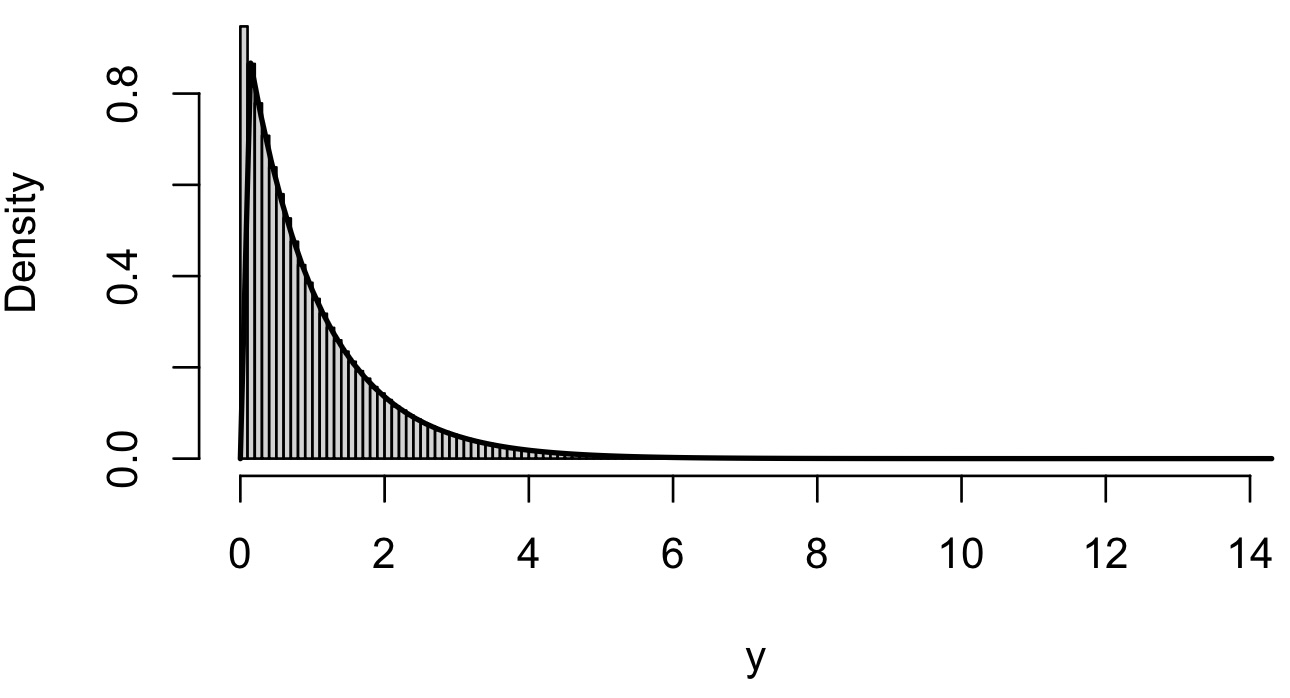
\includegraphics[width=.3\textwidth]{viikko5tehtävä9.jpg}
  \caption{lineaarimuunnos Tas(0,1) -> Tas(a,b)}
\end{figure}
    
\end{comment}



\pagebreak
\item Muokkaa koodia siten, että muunnosfunktio onkin \texttt{y =
-log(x)} (R:ssä pelkkä \texttt{log(x)} tarkoittaa luonnollista logaritmia).
Aja koodi ja tutki histogrammia.\\[6pt]
Vertaa muotoa eksponenttijakauman Exp(1) tiheysfunktioon.\\[6pt]
Vertaa vielä esim.\ tapahtuman $Y\leq 2$ suhteellista frekvenssiä
(\texttt{sum(y<=2)/n}) kyseisen tapahtuman todennäköisyyteen, jos
$Y\sim\operatorname{Exp}(1)$.

\begin{verbatim}
n <- 1e6
x <- runif(n)
y <- -log(x)

hist(y, breaks=120, freq=FALSE)
curve(dexp(x, rate=1), add=TRUE, lwd=2)

# empiirinen P(Y <= 2) ja teoreettinen vertailuarvo
mean(y <= 2)        # [1] 0.865345
pexp(2, rate = 1)   # [1] 0.8646647
\end{verbatim}

\textit{Kommentti.} Koska $X\sim\mathrm{Tas}(0,1)$ ja $Y=-\log X$, niin $y\ge0$:
\[
F_Y(y)=P(Y\le y)=P(-\log X\le y)=P\!\big(X\ge e^{-y}\big)
=1-e^{-y}
\]
Derivoimalla $f_Y(y)=e^{-y},\ y\ge0$, joten $Y\sim\mathrm{Exp}(1)$.
Teoreettinen arvo on siis
\[
P(Y\le 2)=F_Y(2)=1-e^{-2}\approx 0.8647
\]
Simulaatiossa mean(y <= 2) tuottaa hyvin lähellä olevan luvun, ja
hist(y) mukailee piirrettyä dexp käyrää.

\begin{figure}[h]
  \centering
  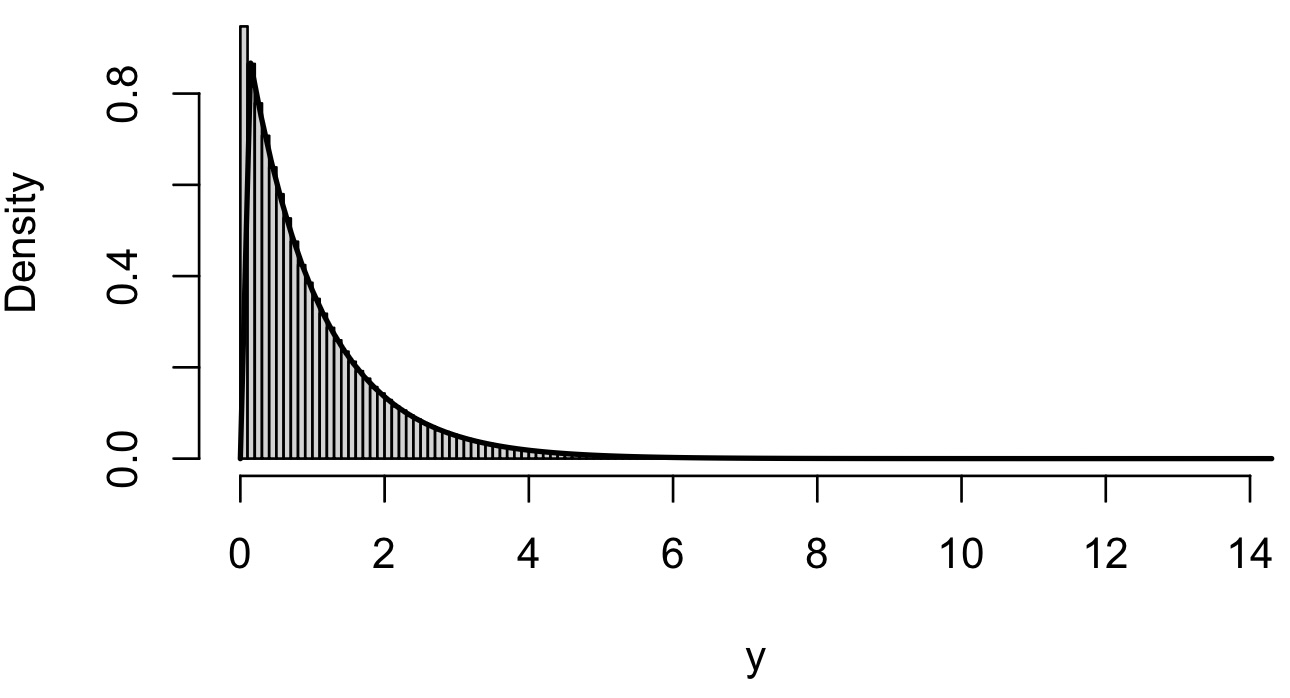
\includegraphics[width=.8\textwidth]{viikko5tehtävä9.jpg}
  \caption{Y = -log(X)}
\end{figure}

\end{kohta}


\end{document}